\chapter{Introduction (10)}

Ernest Rutherford directed a beam of alpha particles (helium nuclei) at a very thin gold foil and observed the scattering pattern on a fluorescent screen which shows the majority of the atom's mass and all of its positive charge was concentrated in a very small central region, which he termed the nucleus.  This was contrary to the then-prevalent 'plum pudding' model proposed by J.J. Thomson, which depicted the atom as a diffuse cloud of positive charge in which the electrons were embedded. Rutherford's nuclear model of the atom, with a dense, positively-charged nucleus surrounded by a cloud of electrons, marked a paradigm shift in our understanding of atomic structure.

[probably not very proper to be here.. to be checked] 

[add binding energy? increase until 26Fe, and drop down, figure of the binding energy]

Our modern understanding shows, at the heart of nuclear structure studies is the nucleus itself, an incredibly dense region at the center of an atom, composed of two types of particles: protons and neutrons, collectively known as nucleons. Despite its small size - typically around 100,000 times smaller than the atom it resides in - the nucleus contains virtually all of the atom's mass. The strong interaction which has a small range but strange force binds neutrons and protons to create atomic nuclei, overcoming the electromagnetic repulsion between protons. The strong interaction is approximately 100 times as strong as electromagnetism, while it has a range of $10^{-15}m$, which is just slightly more than the radius of a nucleon. The strong interaction will only affect adjacent nucleons while the EM force has an unlimited range but with a small force. At small nucleons (A) range, the neutron and proton have almost the same. For a nucleus with larger nucleons, there will be more neutrons than protons. 

\begin{figure}
    \centering
    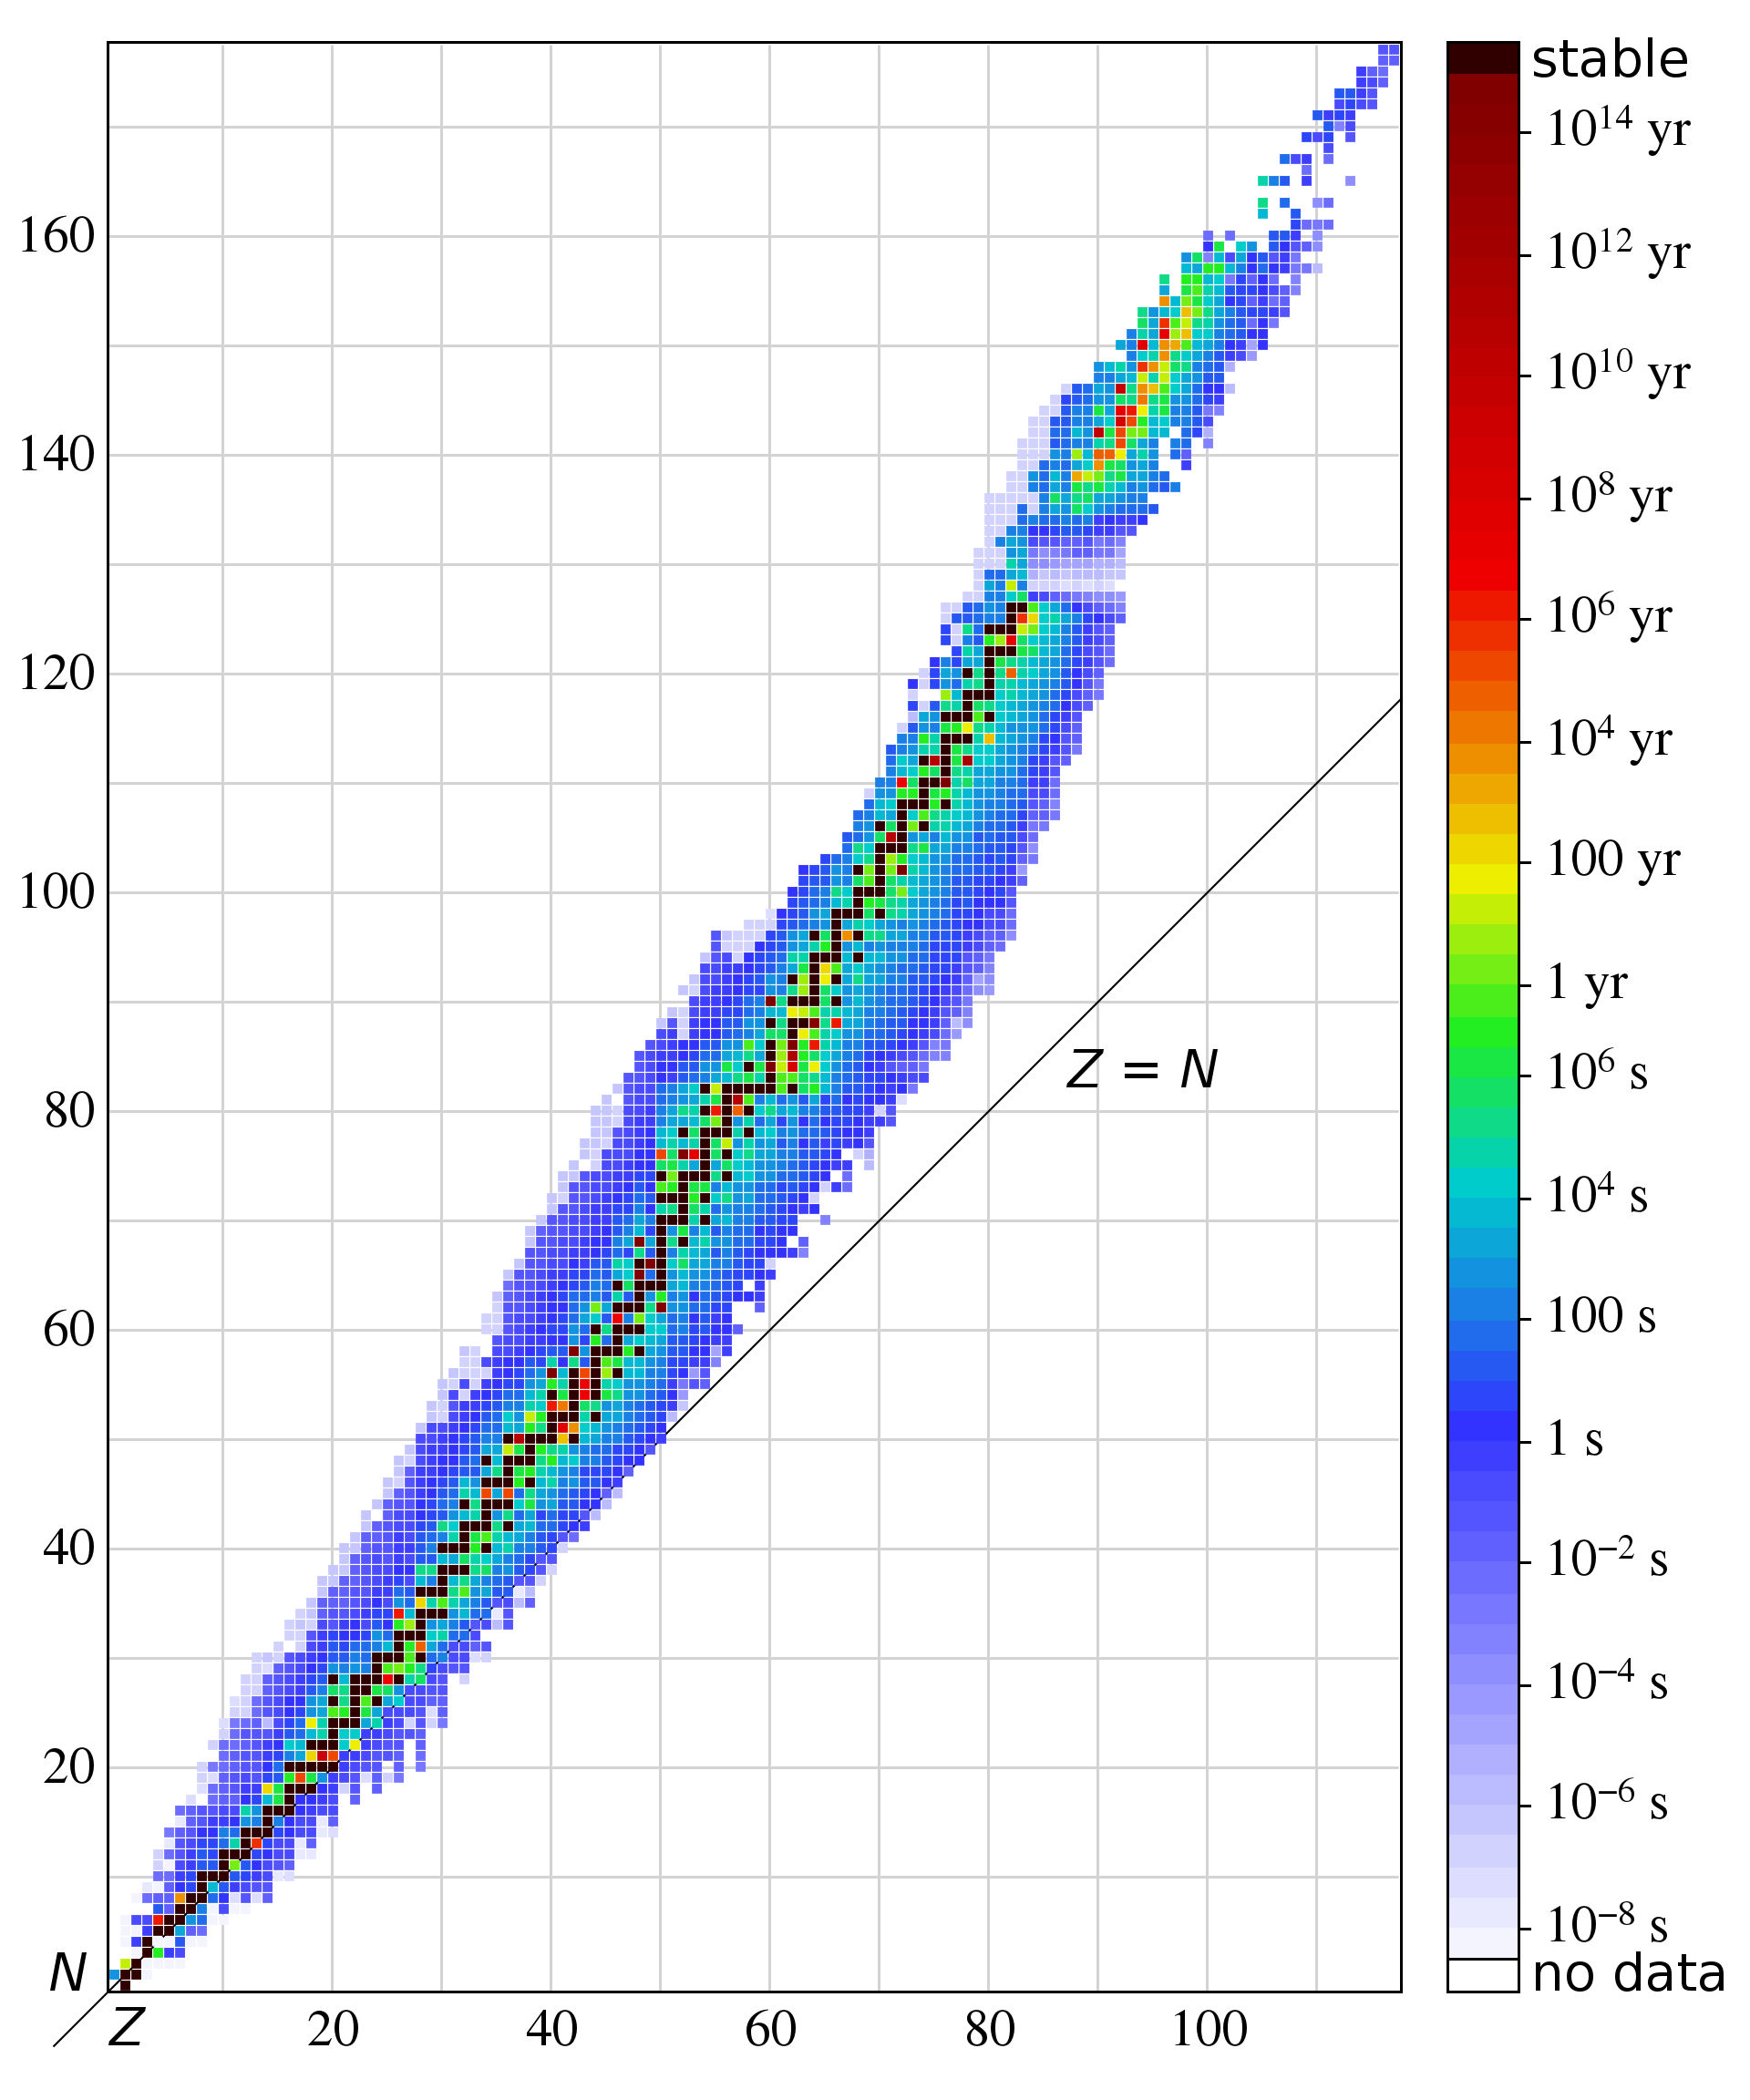
\includegraphics[width=0.8\textwidth]{images/chap1/Isotopes_and_half-life.svg.png}
    \caption{Caption .... plot from wiki}
    \label{fig:isotopes_proton_neutron_ratio}
\end{figure}


In 1961, Robert Hofstadter won Nobel Price for his pioneering studies of the structure of nucleons with electron scattering. Accelerated electron beams have been widely used to study the inner structure of the nucleons (and neutrons) since then. That experiment can provide different level structure information of nucleons given different incident electron energy. At the range where the energy of electrons is deficient, $\lambda \gg r_p$, here $r_p$ is the proton's radius, $\lambda$ is the electron wavelength, the scattering is equivalent to scattered over point like spin-less object. At a low electron energy range where $\lambda ~r_p$, the scattering is equivalent to scattering over the charged object. When the electron wavelength $\lambda < r_p$, the electron scattering will be able to see the substructures. At a very high energy range where $\lambda \ll r_p$, the electrons are equivalent to scattering over the sea of quarks and gluons of the protons. 

[.... to be polished]

A nucleus's root-mean-square (RMS) radius is a key parameter in nuclear physics. It defines the spread of the distribution of nucleons (protons and neutrons) within an atomic nucleus, providing insights into the structure and spatial dimensions of the nucleus. Proton carries charges, it defines the charge radius of the nucleus. The charge radius has been well studied for varieties of isotopes through varieties of experiment methods like electron scattering, and spectroscopy of atomic hydrogen.  In electron scattering experiments, a beam of high-energy electrons is fired at atomic nuclei. By studying the scattering patterns and angles, one can infer information about the charge distribution in the nucleus. Hydrogen spectroscopy, on the other hand, involves measuring the energy levels of hydrogen atoms, which are sensitive to the nuclear charge distribution. This method has been especially significant in the precise determination of the proton charge radius. More recently, the advent of laser spectroscopy has allowed for precise measurements of the charge radii of short-lived isotopes, further expanding our knowledge of nuclear structure.

On the other hand, the precise measurement of the neutron radius is technically challenging due to the nature of the neutron's lack of charge and the need for high-intensity neutron sources. In the theoretical landscape, neutron skin thickness has been studied using a variety of nuclear models, such as the mean field models (including the Relativistic Mean Field and the Skyrme-Hartree-Fock model) and the neutron drop model. These models typically make an assumption that nuclear matter is charge-independent and charge-symmetric, but the asymmetry between the neutron and proton distributions leads to a modification of the standard model. 

[.... add the Skyrme model plot]


Several experiments have been designed to measure the neutron radius or skin thickness. Electron scattering experiments, where high-energy electrons are fired at a target nucleus and their deflection is measured, provide a method to explore the charge distribution and, indirectly, the neutron distribution. Proton scattering experiments can provide more direct information about the neutron distribution. The PREX (Lead Radius Experiment) at Jefferson Lab, for instance, is an experiment designed to measure the neutron radius of lead-208 using parity-violating electron scattering, providing a clean probe of neutron density.


The measurement of the neutron skin has far-reaching implications. On a microscopic level, it provides insights into the equation of state (EoS) of neutron-rich nuclear matter, specifically the symmetry energy, which characterizes how the energy of nuclear matter responds to variations in the neutron-proton ratio. On a macroscopic scale, symmetry energy plays a crucial role in predicting the properties of neutron stars, ultra-dense objects in space primarily composed of neutrons. Hence, the neutron radius study creates a bridge between the smallest scales (atomic nuclei) and the largest scales (neutron stars and supernovae) in the universe.

\section{present knowledge of neutron skin thickness}

In neutron-rich atomic nuclei, the distribution of neutrons extends further than the distribution of protons, leading to a "neutron skin" surrounding the nucleus. The thickness of this neutron skin is determined by the difference in the root-mean-square radii of the neutron and proton distributions. There are several theoretical models and methods used to estimate neutron skin thickness in neutron-rich nuclei.

[need to double check]

\subsubsection{Mean Field Theories}

In Mean Field Theories, each nucleon moves independently in a potential which is an average or "mean" field created by all other nucleons. The most basic version of this is the Hartree-Fock method, where the mean field is determined by the density of the nucleons.

The starting point is the many-body Hamiltonian for a system of nucleons:

\begin{equation}
    H = \sum_i\frac{p_i^2}{2m} + \frac{1}{2}\sum_{i\neq j}v_{ij}
\end{equation}

where $p_i$ is the momentum of the $ith$ nucleon, $m$ is the nucleon mass, and $v_{ij}$ is the interaction potential between the $ith$ and $jth$ nucleons.

In the Hartree-Fock approximation, the many-body wave function of the system is approximated as a Slater determinant, which is an antisymmetrized product of single-particle wave functions. This leads to an effective single-particle Schrödinger equation:

\begin{equation}
    [-\frac{\hbar^2}{2m}\nabla^2 + U(r)]\psi_i(r) = \varepsilon_i\psi(r)
\end{equation}

where $\psi(r)$ is the single-particle wave function, $\varepsilon_i$ is the single-particle energy, and $U(r)$ is the mean field potential, which is determined by the density of the nucleons.

The neutron and proton density distributions, $\rho_n(r)$ and $\rho_p(r)$, are given by the squares of the absolute values of the neutron and proton wave functions, summed over all occupied states:

\begin{equation}
    \rho_n(r) = \sum_{i\in occupied neutron states}|\varepsilon_i(r)|^2
\end{equation}

\begin{equation}
    \rho_p(r) = \sum_{i\in occupied proton states}|\varepsilon_i(r)|^2
\end{equation}


The neutron skin thickness is then given by the difference in the root-mean-square radii of the neutron and proton distributions:

\begin{equation}
    \Delta{R} = \sqrt{<r^2>_n} - \sqrt{<r^2>_p}
\end{equation}

Where. 

\begin{equation}
    <R^2>_{n/p} = \frac{\int{d^3rr^2\rho_{n/p}(r)}}{\int{d^3r\rho_{n/p}(r)}}
\end{equation}

The actual calculations can be quite complex and require numerical methods to solve the Schrödinger equation and to find the density distributions.


\subsubsection{Skyrme-Hartree-Fock Models}

The Skyrme-Hartree-Fock model is a specific type of mean field theory that uses an effective nuclear interaction known as the Skyrme force. The Skyrme force is a phenomenological interaction that has been fitted to nuclear data. It includes terms that represent the kinetic energy of the nucleons, the potential energy due to the interactions between the nucleons, and the exchange energy due to the Pauli exclusion principle.


\subsubsection{Density Functional Theory (DFT)}

Density Functional Theory (DFT) is a quantum mechanical modeling method used in physics and chemistry to investigate the electronic structure (principally the ground state) of many-body systems. In the context of nuclear physics, DFT and its extensions can be used to calculate the neutron skin thickness by minimizing the energy functional with respect to the neutron and proton density distributions.

The starting point is the energy functional, which is a functional of the neutron and proton density distributions, $\rho_p(r)$ and $\rho_p(r)$:

\begin{equation}
    E[\rho_n,\rho_p] = T[\rho_n,\rho_p] + V[\rho_n,\rho_p] + E_{xc}[\rho_n,\rho_p]
\end{equation}

where $T[\rho_n,\rho_p]$ is the kinetic energy functional, $V[\rho_n,\rho_p]$ is the potential energy functional, and $E[\rho_n,\rho_p]$ is the exchange-correlation energy functional, which accounts for the effects of the Pauli exclusion principle and the correlations between the nucleons.

The neutron and proton density distributions are found by minimizing the energy functional with respect to $\rho_n(r)$ and $\rho_p(r)$, subject to the constraints of particle number conservation. This leads to the Kohn-Sham equations, which are a set of single-particle Schrödinger equations:

\begin{equation}
     [-\frac{\hbar^2}{2m}\nabla^2 + U_{n/p}(r)]\psi_{n/p,i}(r) = \varepsilon_{n/p,i}\psi_{n/p,i}(r)
\end{equation}

where $U_n(r)$ and $U_p(r)$ are the effective potentials for the neutrons and protons, respectively, which are given by the functional derivatives of the energy functional with respect to the densities:

\begin{equation}
    U_n(r) = \frac{\delta{E[\rho_n,\rho_p]}}{\delta{\rho_n(r)}}
\end{equation}

\begin{equation}
    U_p(r) = \frac{\delta{E[\rho_n,\rho_p]}}{\delta{\rho_p(r)}}
\end{equation}

\subsubsection{Chiral Effective Field Theory (EFT)}

Chiral Effective Field Theory is a theoretical framework that is based on the symmetries of quantum chromodynamics (QCD), the theory of strong interactions. In this framework, the nucleons (protons and neutrons) and pions (another type of subatomic particle) are treated as effective degrees of freedom, and their interactions are described by an effective Lagrangian.

The starting point is the effective Lagrangian, which is given by:

\begin{equation}
    \mathcal{L} =\mathcal{L}_0 + \mathcal{L}_1 + \mathcal{L}_2 + ...
\end{equation}

where $\mathcal{L}_0$ is the leading-order Lagrangian, $\mathcal{L}_1$ is the next-to-leading-order Lagrangian, $\mathcal{L}_2$ is the next-to-next-to-leading-order Lagrangian, and so on. Each term in the Lagrangian includes interactions between the nucleons and pions that are consistent with the symmetries of QCD.

The neutron and proton density distributions, $\rho_n(r)$ and $\rho_n(r)$, are found by solving the equations of motion derived from the effective Lagrangian. These are typically complex integro-differential equations that require sophisticated numerical methods to solve.

\section{Rich Physics Behind the PRex Experiment}

\subsection{Neutron skin thickness and Neutron Stars}

The neutron skin thickness of a heavy nucleus and the equation of state (EOS) of neutron-rich matter are related through the pressure of neutron-rich matter at the saturation density. This is because both the neutron skin thickness and the pressure depend on the symmetry energy, which describes how the energy of nuclear matter changes when the number of neutrons is not equal to the number of protons.

The pressure $P$ of neutron-rich matter at the saturation density $\rho_0$ is given by,

\begin{equation}
    P = \rho^2\frac{\partial{E/N}}{\partial{\rho}} = \rho_0\frac{S}{3}(2-\frac{L}{3S})
\end{equation}

Here in the equation, $S$ is the symmetry energy, $L$ is the slope of the symmetry energy at $\rho_0$.

\begin{equation}
    L  = 3\rho_0\frac{\partial{S}}{\partial{\rho}}
\end{equation}

The neutron skin thickness $\Delta{R}$ of a heavy nucleus is related to the symmetry energy and its slot by:"

\begin{equation}
    \Delta{R} = \frac{R}{3}\frac{r_0} {c}(\frac{S}{E_{Fermi}} + \frac{L}{3S})
\end{equation}

where $R$ is the radius of the nucleus, $r_0$ is the radius of a nucleon, $c$ is the speed of light, and $E_{Fermi}$ is the Fermi energy.

By measuring the neutron skin thickness and using theoretical models to calculate the symmetry energy and its slope, we can infer the pressure of neutron-rich matter at the saturation density. This provides a constraint on the EOS of neutron-rich matter, which is crucial for understanding the properties of neutron stars.

\subsection{Atomic Parity Violation Experiment}

Atomic parity non-conservation (PNC) studies are sensitive to the neutron skin thickness of heavy nuclei. This is because the PNC effect in heavy atoms is largely due to the weak charge of the nucleus, which is given by the difference between the number of neutrons and protons. The neutron skin thickness is a measure of this difference in the spatial distribution of neutrons and protons.

The PNC effect is observed in the interference between the electromagnetic and weak interactions in atomic transitions. The weak interaction violates parity, which means it can distinguish between a state and its mirror image. This leads to a small asymmetry in the probabilities of certain atomic transitions.

By measuring the PNC effect and the neutron skin thickness, we can infer the weak charge of the nucleus. This provides a test of the standard model of particle physics, which predicts the value of the weak mixing angle.

Furthermore, the PNC effect is sensitive to the distribution of neutrons and protons in the nucleus. Therefore, measurements of the PNC effect can provide information about the neutron skin thickness, which is important for understanding the properties of neutron-rich matter and neutron stars.

\subsection{Heavy ion collisions }
[ref to Isospin Diffusion in Heavy-Ion Collisions and the Neutron Skin Thickness of Lead, need to double check]

Isospin diffusion in heavy-ion collisions and the neutron skin thickness of lead are closely related because they both involve the behavior of neutron-rich matter.

Isospin diffusion is a phenomenon that occurs in collisions between heavy ions, where the neutron-proton asymmetry, or isospin, of the colliding nuclei changes due to the exchange of nucleons between the nuclei. This process is sensitive to the isospin-dependent part of the nuclear interaction, which is also related to the neutron skin thickness.

The neutron skin thickness of a heavy nucleus like lead-208 is a measure of the neutron-proton asymmetry in the spatial distribution of nucleons in the nucleus. A larger neutron skin thickness indicates a larger neutron-proton asymmetry.

In heavy-ion collisions, the isospin diffusion can be described by the equation:

\begin{equation}
    \frac{d\delta}{d t} = - \frac{1}{\tau}\delta
\end{equation}

where $\delta$ is the isospin asymmetry and ττ is the isospin relaxation time. The relaxation time $\tau$ is related to the isospin-dependent part of the nuclear interaction, which is also related to the neutron skin thickness.


\section{The Previous Experiment}


The Lead Radius Experiment The experiment used a beam of high-energy electrons to probe the lead-208 nucleus. The electrons were polarized, meaning they had a preferred spin direction. This allowed the experiment to take advantage of the weak force, which violates parity and thus can distinguish between neutrons and protons. The electrons scattered off the lead-208 nucleus, and the scattered electrons were detected. By measuring the asymmetry in the scattering of the polarized electrons, the experiment was able to determine the neutron skin thickness.

The results of the PREX-I experiment provided a direct measurement of the neutron skin thickness of lead-208. This was a significant achievement, as previous measurements had relied on indirect methods. The results of the PREX-I experiment have important implications for our understanding of neutron-rich matter and neutron stars. The neutron skin thickness is closely related to the equation of state of neutron-rich matter, which determines many properties of neutron stars.

The PREX-I experiment faced several challenges, including statistical uncertainties and systematic errors. The measurement of the neutron skin thickness is a difficult task that requires high precision and accuracy.  Following the success of the PREX-I experiment, a second experiment, PREX-II, was proposed to further refine the measurement of the neutron skin thickness of lead-208. The PREX-II experiment aims to reduce uncertainties and improve the precision of the measurement.

Besides that, another sister experiment 'CRex' experiment was also proposed which performed at exactly the same condition but at different beam energy and target. 

\begin{itemize}
    \item PRex and result
\end{itemize}

\begin{itemize}
    \item PRex-II experiment 
\end{itemize}

\begin{itemize}
    \item CRex experiment
\end{itemize}


\section{Impact of the experiment, result based on PRex-II experiment [move to chapter 6 conclusion]}

\subsection{calculate with Coulomb energy differences Phys. Lett 29B 396 (1969)}
\subsection{L. Ray and G.W.Hoffmann Physics Rev C 31. 538 (1985)}